\chapter{Classical Computations}
The Turing Machine is an abstract model of computation that can perform any computation that can be performed by a digital computer. It is a mathematical model of computation that defines an abstract machine which manipulates symbols on a strip of tape according to a table of rules.
The machine operates on an infinite memory tape divided into discrete cells. Each cell contains a symbol from a finite alphabet. The machine has a read/write head that can read the symbol on the tape and write a new symbol. The machine can move the tape left or right one cell at a time. The machine has a finite set of states and a table of rules that determine the next state of the machine based on the current state and the symbol read from the tape. The machine halts when it reaches a halting state. The Turing Machine can perform any computation that can be performed by a digital computer. It is a universal 
model of computation that can simulate any other computational model.

But in real world, the computers are finite in size.
An alternative model of computation is the circuit model which is equivalent to the Turing Machine
and is suitable for studying the complexity of algorithms. The circuit model consists of gates that perform logical operations on bits. The gates are connected by wires that carry the bits from one gate to another. 
The circuit model can be used to represent any computation that can be performed by a 
digital computer. The circuit model is a useful abstraction that 
allows us to reason about the efficiency of algorithms and design better algorithms. 

\begin{definition}
\textbf{Logic Gate: }It is a function defined as $f:\{0,1\}^k \rightarrow \{0,1\}^l$ where k is the number of input bits and 
l is the number of output bits.
\end{definition}
Note that no loops are allowed in such circuits to avoid instabilities. Thus, they are Acyclic circuits.
This is the Circuit Model of Computation.
Some of the useful Logic Gates are:
\section{Classical Logic Gates}
\subsection{NOT Gate}\label{cgate:NOT}
The NOT gate is a unary gate that takes a single input bit and produces a single output bit. The output bit is the complement of the input bit i.e. if the input bit is 0, the output bit is 1 and if the input bit is 1, the output bit is 0.
The truth table for the NOT gate is:
\begin{table}[ht]
    \centering
    \begin{tabular}{|c|c|}
        \hline
        Input & Output \\
        \hline
        0 & 1 \\
        1 & 0 \\
        \hline
    \end{tabular}
    \caption{Truth table for NOT Gate}
    \label{tab:NOT_GATE}
\end{table}

The NOT gate is denoted by the symbol $\neg$.
It's symbol is as shown:
\begin{center}
    \begin{circuitikz}
        \draw (0,0) node[not port] (mynot) {};
    \end{circuitikz}
\end{center}
Mathematically, the NOT gate is defined as:
\[ f(x)=\neg x \]

\subsection{AND Gate}\label{cgate:AND}
The AND gate is a binary gate that takes two input bits and produces a single output bit. The output bit is 1 if both input bits are 1 and 0 otherwise.
The truth table for the AND gate is:
\begin{table}[ht]
\centering
    \begin{tabular}{|c|c|c|}
        \hline
        Input 1 & Input 2 & Output \\
        \hline
        0 & 0 & 0 \\
        0 & 1 & 0 \\
        1 & 0 & 0 \\
        1 & 1 & 1 \\
        \hline
    \end{tabular}
    \caption{Truth table for AND Gate}
    \label{tab:AND_GATE}
\end{table}
The AND gate is denoted by the symbol $\land$.
It's symbol is as shown:
\begin{center}
    \begin{circuitikz}
        \draw (0,0) node[and port] (myand) {};
    \end{circuitikz}
\end{center}
Mathematically, the AND gate is defined as:
\[ f(x,y)=x \land y \]

\subsection{OR Gate}
The OR gate is a binary gate that takes two input bits and produces a single output bit. The output bit is 1 if at least one of the input bits is 1 and 0 otherwise.
The truth table for the OR gate is:
\begin{table}[ht]
\centering
    \begin{tabular}{|c|c|c|}
        \hline
        Input 1 & Input 2 & Output \\
        \hline
        0 & 0 & 0 \\
        0 & 1 & 1 \\
        1 & 0 & 1 \\
        1 & 1 & 1 \\
        \hline
    \end{tabular}
    \caption{Truth table for OR Gate}
    \label{tab:OR_GATE}
\end{table}
The OR gate is denoted by the symbol $\lor$.
It's symbol is as shown:
\begin{center}
    \begin{circuitikz}
        \draw (0,0) node[or port] (myor) {};
    \end{circuitikz}
\end{center}
Mathematically, the OR gate is defined as:
\[ f(x,y)=x \lor y \]

\subsection{NAND Gate}
The NAND gate is a binary gate that takes two input bits and produces a single output bit. The output bit is the complement of the AND gate i.e. the output bit is 0 if both input bits are 1 and 1 otherwise.
The truth table for the NAND gate is:
\begin{table}[ht]
\centering
    \begin{tabular}{|c|c|c|}
        \hline
        Input 1 & Input 2 & Output \\
        \hline
        0 & 0 & 1 \\
        0 & 1 & 1 \\
        1 & 0 & 1 \\
        1 & 1 & 0 \\
        \hline
    \end{tabular}
    \caption{Truth table for NAND Gate}
    \label{tab:NAND_GATE}
\end{table}
The NAND gate is denoted by the symbol $\overline{\cdot}$.
It's symbol is as shown:
\begin{center}
    \begin{circuitikz}
        \draw (0,0) node[nand port] (mynand) {};
    \end{circuitikz}
\end{center}
Mathematically, the NAND gate is defined as:
\[ f(x,y)=\neg (x \land y) \]
Note that the NAND Gate can also be written by adding a NOT gate at the output of the AND gate as shown:
\begin{center}
    \begin{circuitikz}
        \draw (0,0) node[and port] (myand) {};
        \draw (myand.out) -- ++(1,0) node[not port] (mynot) {};
    \end{circuitikz}
\end{center}

\subsection{NOR Gate}
The NOR gate is a binary gate that takes two input bits and produces a single output bit. The output bit is the complement of the OR gate i.e. the output bit is 0 if at least one of the input bits is 1 and 1 otherwise.
The truth table for the NOR gate is:
\begin{table}[ht]
\centering
    \begin{tabular}{|c|c|c|}
        \hline
        Input 1 & Input 2 & Output \\
        \hline
        0 & 0 & 1 \\
        0 & 1 & 0 \\
        1 & 0 & 0 \\
        1 & 1 & 0 \\
        \hline
    \end{tabular}
    \caption{Truth table for NOR Gate}
    \label{tab:NOR_GATE}
\end{table}
The NOR gate is denoted by the symbol $\overline{A\lor B}$
It's symbol is as shown:
\begin{center}
    \begin{circuitikz}
        \draw (0,0) node[nor port] (mynor) {};
    \end{circuitikz}
\end{center}
Mathematically, the NOR gate is defined as:
\[ f(x,y)=\neg (x \lor y) \]
NOR Gate can also be written by adding a NOT gate at the output of the OR gate as shown:
\begin{center}
    \begin{circuitikz}
        \draw (0,0) node[or port] (myor) {};
        \draw (myor.out) -- ++(1,0) node[not port] (mynot) {};
    \end{circuitikz}
\end{center}

\subsection{XOR Gate}
The XOR gate is a binary gate that takes two input bits and produces a single output bit. The output bit is 1 if the input bits are different and 0 otherwise.
The truth table for the XOR gate is:
\begin{table}[ht]
\centering
    \begin{tabular}{|c|c|c|}
        \hline
        Input 1 & Input 2 & Output \\
        \hline
        0 & 0 & 0 \\
        0 & 1 & 1 \\
        1 & 0 & 1 \\
        1 & 1 & 0 \\
        \hline
    \end{tabular}
    \caption{Truth table for XOR Gate}
    \label{tab:XOR_GATE}
\end{table}
The XOR gate is denoted by the symbol $\oplus$.
It's symbol is as shown:
\begin{center}
    \begin{circuitikz}
        \draw (0,0) node[xor port] (myxor) {};
    \end{circuitikz}
\end{center}
Mathematically, the XOR gate is defined as:
\[ f(x,y)=x \oplus y \]

\subsection{FANOUT Gate}
The FANOUT gate is a unary gate that takes a single input bit and produces two output bits. The output bits are the same as the input bit.
The truth table for the FANOUT gate is:
\begin{table}[ht]
\centering
    \begin{tabular}{|c|c|c|}
        \hline
        Input & Output 1 & Output 2 \\
        \hline
        0 & 0 & 0 \\
        1 & 1 & 1 \\
        \hline
    \end{tabular}
    \caption{Truth table for FANOUT Gate}
    \label{tab:FANOUT_GATE}
\end{table}
Mathematically, the FANOUT gate is defined as:
\[ f(x)=(x,x) \]

\subsection{CROSSOVER Gate}
The CROSSOVER gate is a binary gate that takes two input bits and produces two output bits. The output bits are the complement of the input bits i.e. if the input bits are (0,1), the output bits are (1,0) and if the input bits are l, the output bits are (0,1).
The truth table for the CROSSOVER gate is:m
\begin{table}[ht]
\centering
    \begin{tabular}{|c|c|c|c|c|}
        \hline
        Input 1 & Input 2 & Output 1 & Output 2 \\
        \hline
        0 & 0 & 0 & 0 \\
        0 & 1 & 1 & 0 \\
        1 & 0 & 0 & 1 \\
        1 & 1 & 1 & 1 \\
        \hline
    \end{tabular}
    \caption{Truth table for CROSSOVER gate}
    \label{tab:CROSSOVER_GATE}
\end{table}
This is same as saying that the value of two bits are interchanged.

Note that OR gate can be simulated by three NOT gates and one AND gate using \textbf{De Morgan's law}
\[
a\lor b=\neg(\neg a\land \neg b) 
\]
Similarly XOR gate can be simulated by AND and NOT gates as
\[
a \oplus b=(\neg a \land b) \lor (a\land \neg b)
\]
which can be further simplified by using the above definition of OR gate using AND and NOT gate.

\section{Classical Circuits}
\begin{definition}
    \textbf{Ancilla bits: }The Ancilla or work bits are the extra bits that are used in the computation 
to store the intermediate results. They are temporary storage devices
that is used to store the intermediate results are are not a part of the inputs 
or the output bits of the computation.
\end{definition}
\begin{theorem}
There always exists a classical circuit which can simulate any classical boolean function $f$.
\end{theorem}
\label{proof:classicalcomputations}
\begin{proof}
    Any fixed gates can be used to compute any function $f:\{0,1\}^n \rightarrow \{0,1\}^m$.
    Consider the proof for the simplified function $f:\{0,1\}^n \rightarrow \{0,1\}$ with n input bits
    and a single output bit. This is a Boolean function. Using mathematical induction, For $n=1$, there are four possible functions: the identity, which is 
    a single wire; the bit flip, implemented using a NOT Gate; the function which replaces the input bit with a 0, which can be obtained using ANDing the input 
    with a work bit initially in the 0 state; and the function which replaces the input bit with a 1, which can be obtained using ORing the input with a work bit initially in the 1 state.
    Thus, we have proved for n=1.
    
    Now for some n, suppose that any function on n bits may be computed by a circuit and let $f$ be a function on $n+1$ bits. 
    Define $f_0$ and $f_1$ to be the functions on n bits obtained by fixing the last bit of the input to 0 and 1 respectively.
    So $f_0=f(x_1,x_2,\ldots,x_n,0)$ and $f_1=f(x_1,x_2,\ldots,x_n,1)$.
    By the induction hypothesis, there are circuits $C_0$ and $C_1$ that compute $f_0$ and $f_1$ respectively.
    Thus, now we are required to design a circuit with computes $f$. Thus, we design a circuit that computes both $f_0$ and $f_1$ 
    on the first n bits and then depending on whether the first bit of the input was 0 or a 1 it outputs the appropriate answer.
    This can be done using a circuit as shown in figure \ref{fig:compute}.
    \begin{figure}[ht]
        \centering
        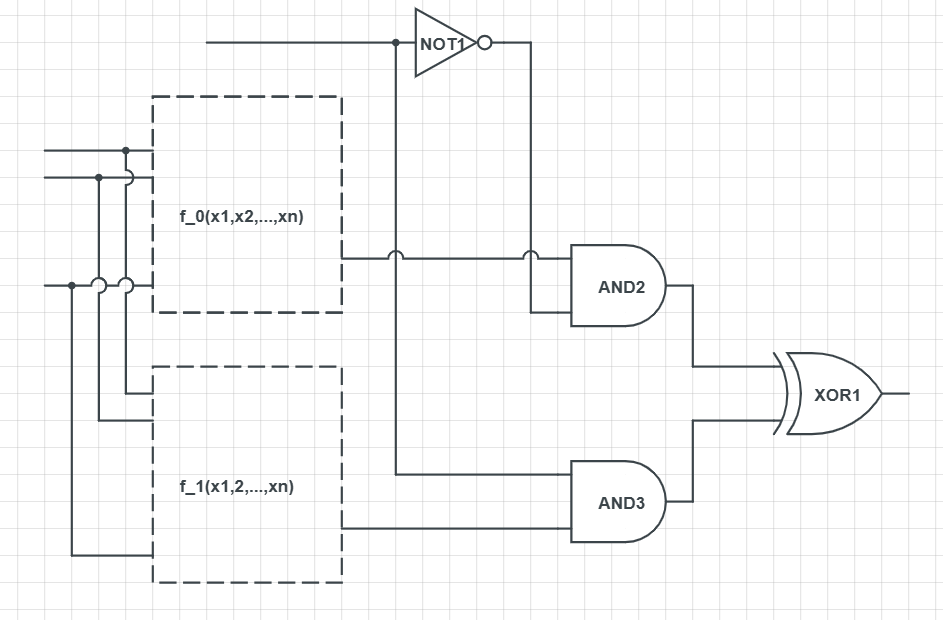
\includegraphics[width=0.8\textwidth]{Images/compute.png}
        \caption{Circuit to compute $f$}
        \label{fig:compute}
    \end{figure}
\end{proof}
For the Universal Circuit Construction:
\begin{itemize}
    \item wires, which preserve the states of the bits;
    \item ancilla bits prepared in the standard states, used in the n=1 case of the proof;
    \item FANOUT operation, which takes a single bits as input and outputs two copies of that bit;
    \item The CROSSOVER operation, which interchanges the values of the two bits;
    \item the AND, OR, and NOT operations, which are the basic logic gates.
\end{itemize}

In the case of quantum wires for the preservation of qubits qubit state, it is not necessarily obvious that good quantum wires for
the preservation of qubits can be constructed. The FANOUT operation cannot be performed because of the \textbf{No - cloning Theorem}.
The AND and XOR Gates are not invertible thus irreversible and hence can't be implemented in a straight forward manner as unitary quantum gates.
Thus, implementing a universal quantum circuit is not as straight forward as in the classical case.

\begin{example}
    Half adder and Full adder circuits used in Classical Computers.
\end{example}
\section{Classical Algorithms as logic circuits}
We can represent algorithms as logic circuits with the inputs on the left, time flows left to right and the outputs are on the right. Classical computer algorithms usually described in high level languages, but they implicitly represent many low-level logic operations, like this circuit shown in figure \ref{fig:classical-circ} of example.
\begin{figure}
    \centering
    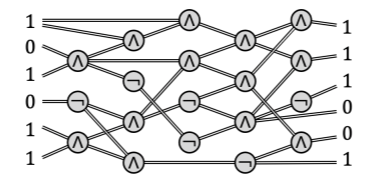
\includegraphics[width=0.5\linewidth]{Images/classical_circ.png}
    \caption{Generic form of a classical circuit (information flows from left to right)}
    \label{fig:classical-circ}
\end{figure}
a reasonable overall cost measure is the number of gates. There are other measures that we may care about such as the \textit{depth}, which is the length of the longest path from an input to an output. Or the \textit{width}, which is the maximum number of gates at any level, assuming that the gates are arranged in levels. But, to keep things simple, let's use the gate count as our main cost measure.

The number of gates depends on what the elementary operations are. We'll take these to be AND and NOT gates (and let's not count the fan-out operations). What's important is that a gate does a constant amount of computational work. If we allowed arbitrary gates then any circuit could be reduced to just one supergate, but the cost of that one gate would not be very meaningful, but since we expect large gates to be expensive to implement.

\subsection{Multiplication problem and factoring problem}
Let's consider the \textit{multiplication problem} where one is given two n-bit binary integers as input and the output is their product (a 2n-bit integer). For example, for inputs 101 and 111, the output should be 100011 (because the product of 5 and 7 is 35).
Think of the number of bits n as being quite large, larger than the number of bits of the arithmetic logic unit of your computer. In principle, you could multiply two numbers consisting of thousands of digits by pencil and paper using the method taught in school. And it can be coded up as an algorithm (commonly referred to as the grade school multiplication algorithm). How efficient is this algorithm? assuming you learned the algorithm that I did, its running time scales quadratically in its input size. By quadratic, I mean some constant times $n^2$ (for sufficiently large n).

The constant depends on the exact gate set that you use and we'll often use the big-oh notation to suppress that.

\begin{definition}
    For $f,g:\mathbb{N}\rightarrow\mathbb{N}, g(n) \in O(g(n))$ if $f(n)\leq cg(n)$ for some constant $c > 0$ (and for sufficiently large n).
\end{definition}
Of course if we want to implement an algorithm then we do care about what the constant multiple is. But if we're looking at things theoretically then the big-oh notation helps reduce clutter and focus attention on asymptotic growth rates, which tend to be more important for large n.

There are more efficient algorithms than the grade school method. The current record is $O(n \log n)$ which is quite good. (There's a rich history of multiplication algorithms that evolved from $O(n^2)$ to $O(n \log n)$, but we won't get into that here).

Now let's look at the factoring problem, which can be roughly thought of as the inverse of the multiplication problem. The input is an n-bit number and the output is its prime factors. For example, for input 100011, the outputs are 101 and 111 (the prime factors of 35).

You probably also learned this algorithm in grade school For factoring numbers: first check it the number is divisible by 2. Then check for divisibility by 3. You can skip 4, since that's a multiple of 2. then check 5, skip 6, check 7m and so on. You can stop once you get to the square root of the number because if you haven't found a divisor by then, the number must be prime.

How expensive is this computationally? For large n, there are a lots of divisors to check, exponentially many. the cost is exponential in n, namely $O(exp(n))$. there are more sophisticated algorithms than this method. The best currently-known classical algorithm for factoring is the so-called \textit{number field sieve algorithm}, which scales exponentially in the cube root of n (to be more precise, $exp(n^{1/3}\log^{2/3}(n))$. since the cube root is in the exponent, this is still essentially exponential. There is no currently-known classical algorithm for factoring whose cost scales polynomially with respect to n.

In fact, the presumed difficulty of factoring is the basis of the security of many crypto-systems.

\section{Classical Circuits}
In classical complexity theory, a Boolean circuit is a finite directed acyclic graph with AND, OR, and NOT gates. It has n input nodes, which contain the n input bits ($n\geq 0$). The internal nodes are AND, OR and NOT gates according to the circuit, and there are one or more designated output nodes. The initial input bits are fed into AND, OR and NOT gates according to the circuit, and eventually the output nodes assume some value.

\textbf{We say that a circuit computes a Boolean function $f:\{0,1\}^n \rightarrow \{0,1\}^m$ if the output nodes get the right value $f(x)$ for every input $x \in \{0,1\}^n$.}

A circuit family is a set $C=\{C_n\}$ of circuits, one for each input size $n$. Each circuit has one output bit. Such a family recognizes or decides a language $L \subseteq \{0,1\}^*=\cup_{n\geq 0} \{0,1\}^n$ if, for every $n$ and every input $x \in \{0,1\}^n$, the circuit $C_n$ outputs 1 if $x \in L$ and outputs 0 otherwise. We can think of language $L$ as a sequence of Boolean functions $f_n:\{0,1\}^n \rightarrow \{0,1\}$, where $f_n$ takes value 1 exactly on the n-bit strings that are in $L$. The circuit $C_n$ then computes the function $f_n$. Such a circuit family is uniformly polynomial if there is a deterministic Turing machine that outputs $C_n$ given n as input, using space logarithmic in $n$. Logarithmic space implies time that's at most polynomial in n, because such a machine will have only $poly(n)$ different internal states, so it either halts after $poly(n)$ steps or cycles forever. Note that the size (number of gates) of the circuit $C_n$ can then grow at most polynomially with $n$. It is known that uniformly polynomial circuit family iff $L\in P$, where $P$ is the class of languages decidable by polynomial-time Turing machines.

Similarly, we can consider randomized circuits. these, receive, in addition to the n input bits, also some random bits ("coin flips") as input. A randomized circuit computes a function $f$ if it successfully computes the right answer $f(x)$ with probability at least $2/3$ for every $x$ (probability taken over the values of the random bits). Randomized circuits are equal in power to randomized Turing machines: a language $L$ can be decided by a uniformly polynomial randomized circuit family iff $L \in BPP$, where $\mathbf{BPP}$ ("Bounded-error Probabilistic Polynomial time") is the class of languages that can efficiently be recognized by randomized Turing machines with success probability at least $2/3$. because we can efficiently reduce the error probability of randomize algorithms, the particular value $2/3$ doesn't really matter here and may be replaced with any fixed constant in $(1/2,1)$.






